\chapter{Results and Discussion}

Our Setup described in Chapter 2 was completed as described in Chapter 3, to collect the building energy requirement in dependence of 324 different panels orientations.\\
The data manipulation is described and then the obtained results are explained.\\
Each simulation provides a .cvs table with the following structure: each row corresponds to an hour of the year and in the five columns the corresponding time, heating, cooling, electricity consumption and room temperature are saved.
This large amount of data is analyzed in MATLAB in the following way:\\
Each parameter (Heating E, Cooling E, Electricity E) is analyzed separately but with the same strategy. All the file-tables are imported as matrixes in MATLAB. The minimization occurs in two steps: first for each combination the vertical rotation with minimal energy is found (see also the \textit{combination Analysis} file in the appendix), then the obtained data are inserted in a new matrix and minimized to find the horizontal combination with minimal energy (see \textit{Overall minimization} in appendix).
The obtained data are visualized (using the file \textit{Minimal plot} in appendix) in the figure display in the following sections.

\newpage

\section{Heating minimization}

The rotations minimizing the heat required by the room are displayed in Figure~\ref{rotation}. Especially in the cold season and in the morning there is a configuration involving many orientations each day, almost each hour required a different orientation from the previous. We remark that the background is blue, corresponding to an orientation of $-75 ^\circ$, not because it required less energy, but because it required the same energy as all other orientations. Two reasons explain this situation: the building requires no additional heat (specially in summer) or the panel orientation doesn't influence the heat required from the building (during the night).\\
The panels follows the sun, but to allow much solar radiation as possible to penetrate inside the building.

\begin{figure}[h]
 \centering
 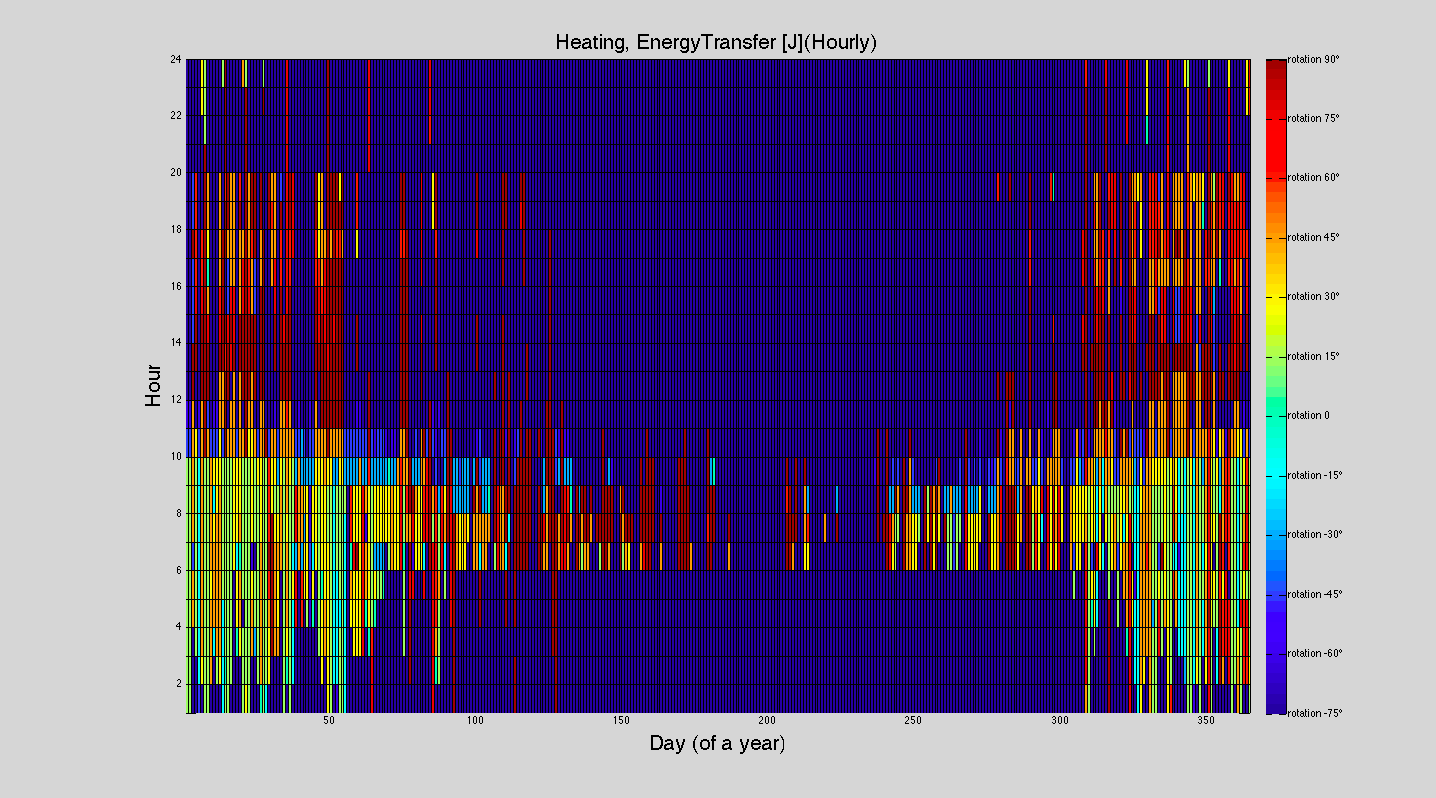
\includegraphics[width=125mm]{graphic/rotation.png}
 \caption{Rotations minimizing the heat required by the room}
 \label{rotation}
\end{figure}

The configurations minimizing the heat required by the room (see Figure~\ref{configuartions}) can be divided in two groups. During the morning the configuration obtained from the minimization is the '222' (green) indicating alls panels are oriented at $45 ^\circ$. During the afternoon, the panels turn to combination '323' (Red) indicating a plain orientation of two rows.

\begin{figure}[h]
 \centering
 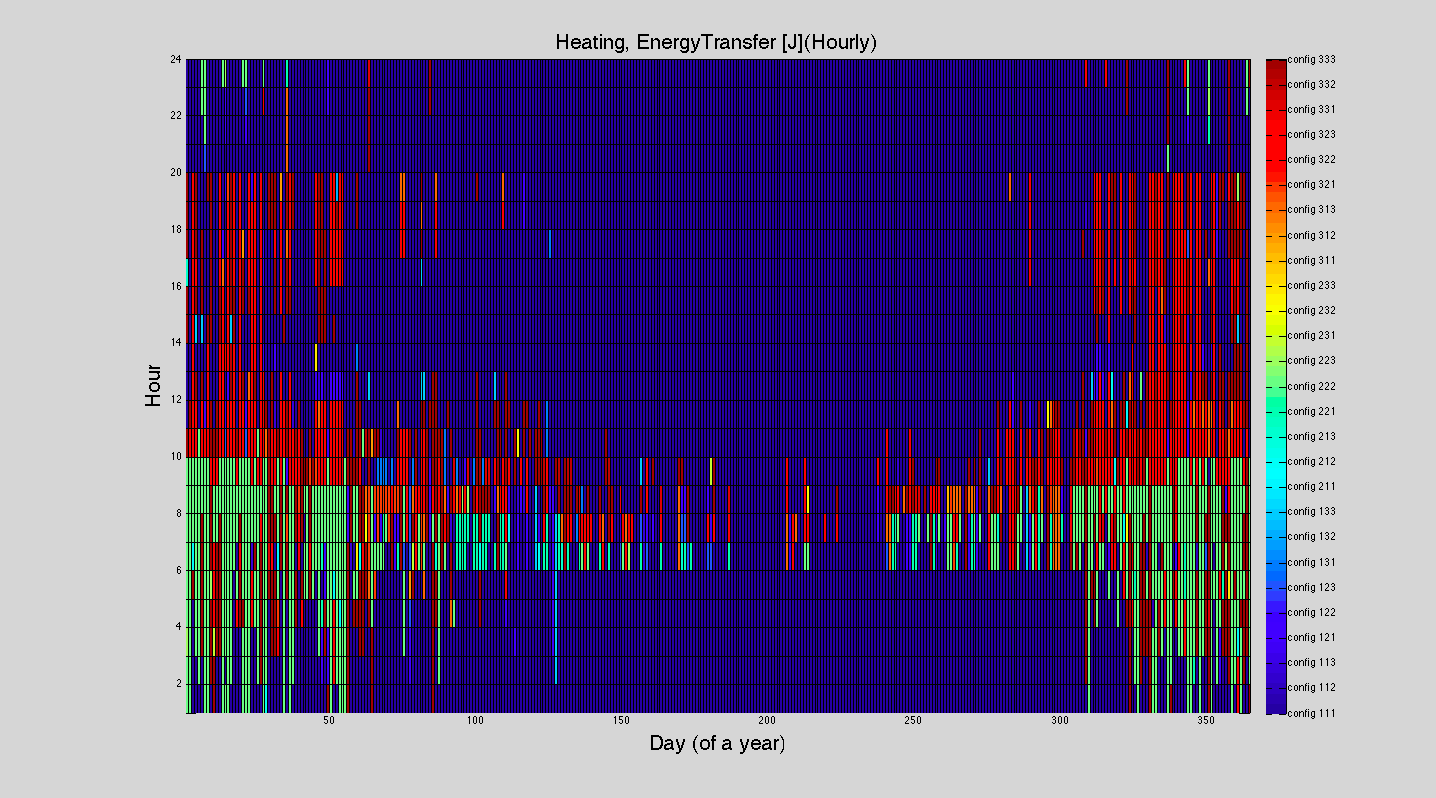
\includegraphics[width=130mm]{graphic/combination.png}
 \caption{Configurations minimizing the heat required by the room}
 \label{configuartions}
\end{figure}

\newpage

\section{Cooling minimization}

Chiefly in the summer afternoon, the panel configuration affect the energy required to cool the building. The configuration '222' is dominating the Figure~\ref{cooling}, this configuration is able to maximize the shading effect.

\begin{figure}[h]
 \centering
 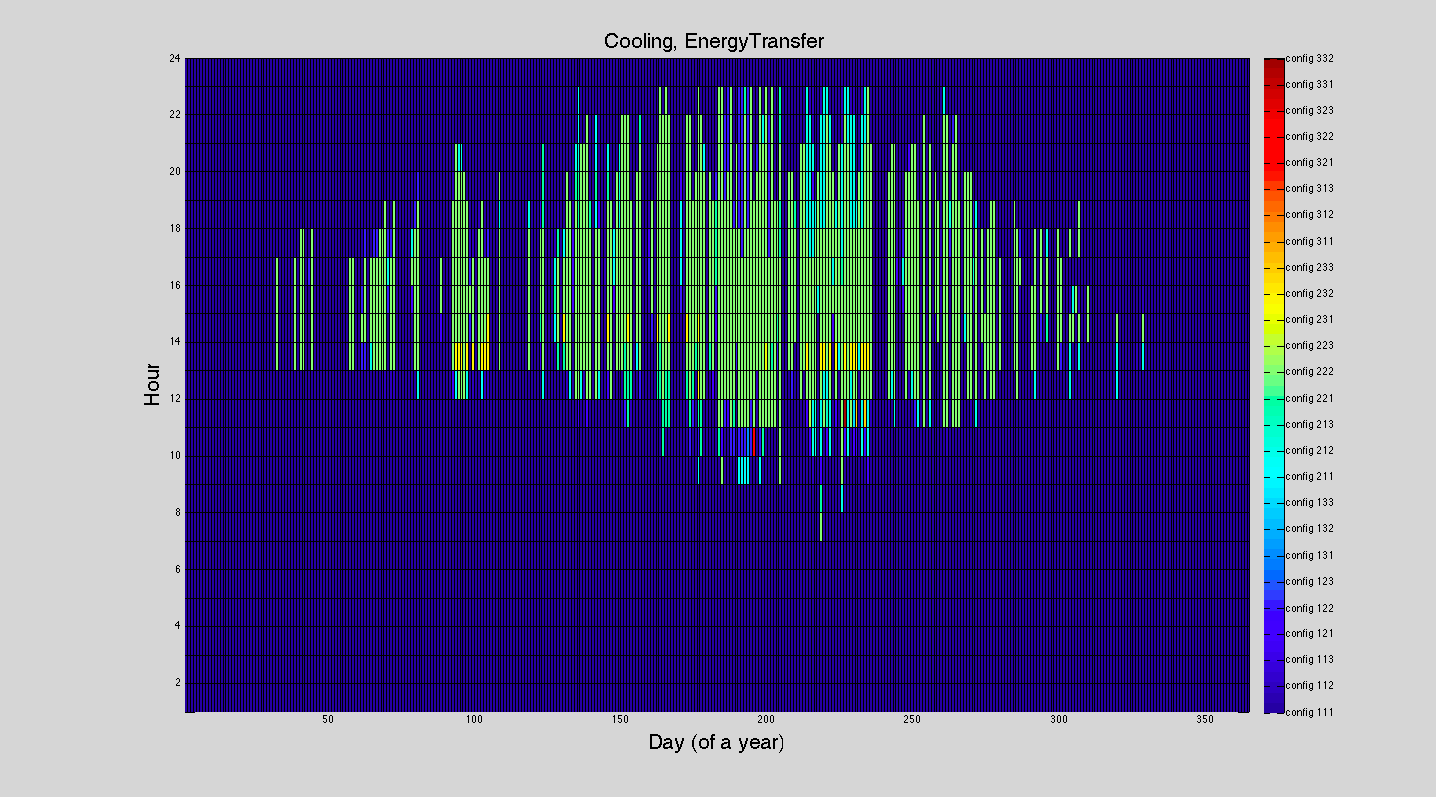
\includegraphics[width=125mm]{graphic/cooling.png}
 \caption{Configurations minimizing the cooling energy required by the room}
 \label{cooling}
\end{figure}

\newpage

\section{Electricity minimization}

The configurations minimizing the electric light (Figure~\ref{light}) are only three. In the middle of the night and day the electric light are off (no occupancy during the night, no electrical light requirement in the middle of the day).\\
Only in the morning and in the evening configurations '333' (red) and '133' (azure) are exploited. This configurations maximize the light crossing the solar adaptive fa\c{c}ade.

\begin{figure}[h]
 \centering
 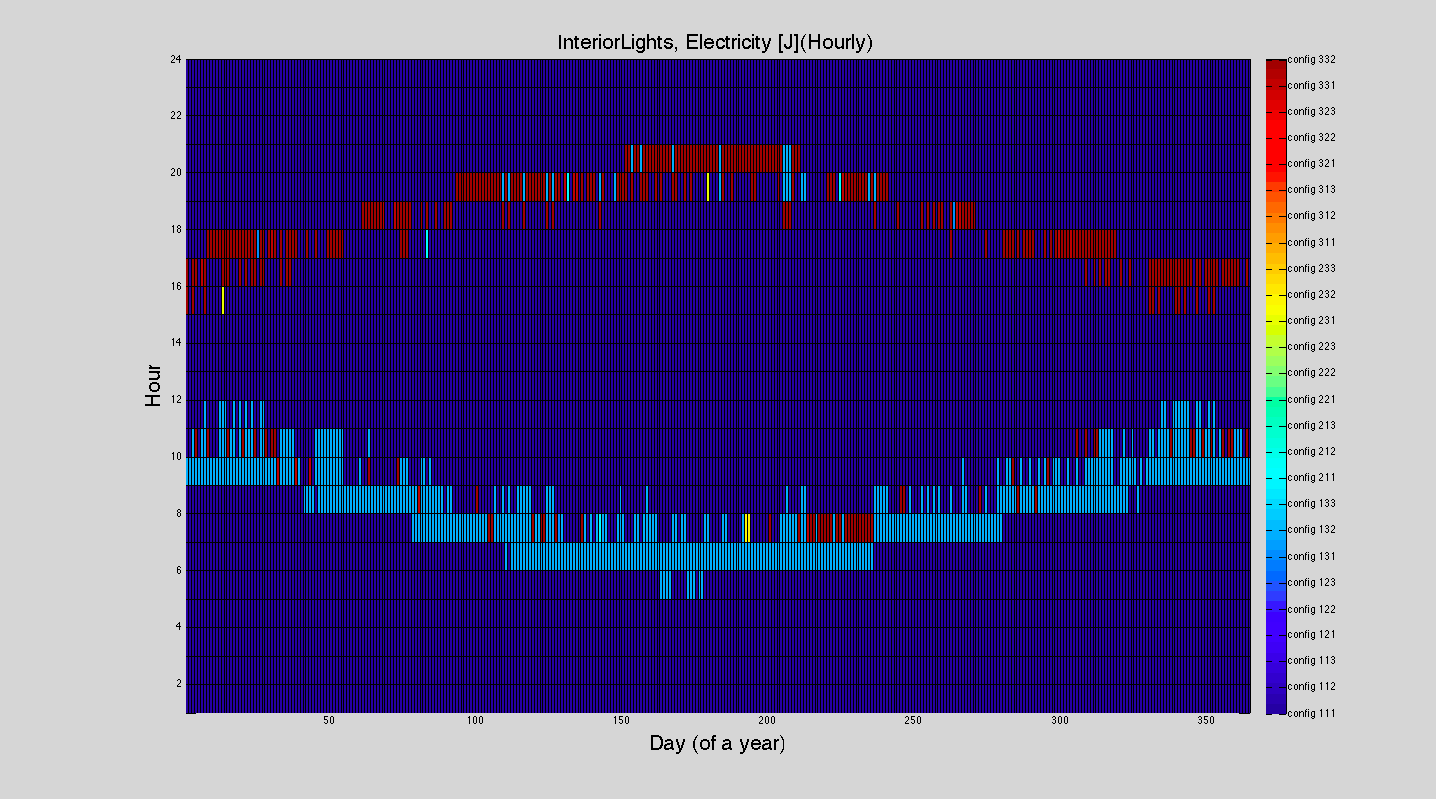
\includegraphics[width=150mm]{graphic/electricity.png}
 \caption{Configurations minimizing the electric light required by the room}
 \label{light}
\end{figure}

\newpage
\section{Visualization}

In order to visualize the results the pictures in Figure~\ref{visualization} have been created using the 'DIVA Daylight Visualization tool'. They compare the results obtained by minimizing the heating (left column), the cooling (middle) and the electricity (right column).
These images are all related to the first of February, this day was chose because it describe a typical day with several different combinations inside (the shadows have the same place at each hour to enphasize the pannels).\\
This visualization highlights non homogeneous solutions: the three bands of panels presents often different orientation from each other. We deduce that the lower panels band has a limited impact on the daylight penetration in the room.\\
The resulting visualization are not easily predictable due to the complexity and the high number of factors which are influenced by. But some common characteristics can be drawn: an open solution provides a reduction in heat and electric light consumption due to increased passive solar irradiation gain, a close solution instead limited the cooling requirement due to reduced passive solar irradiation gain.

\begin{figure}[h]
 \centering
 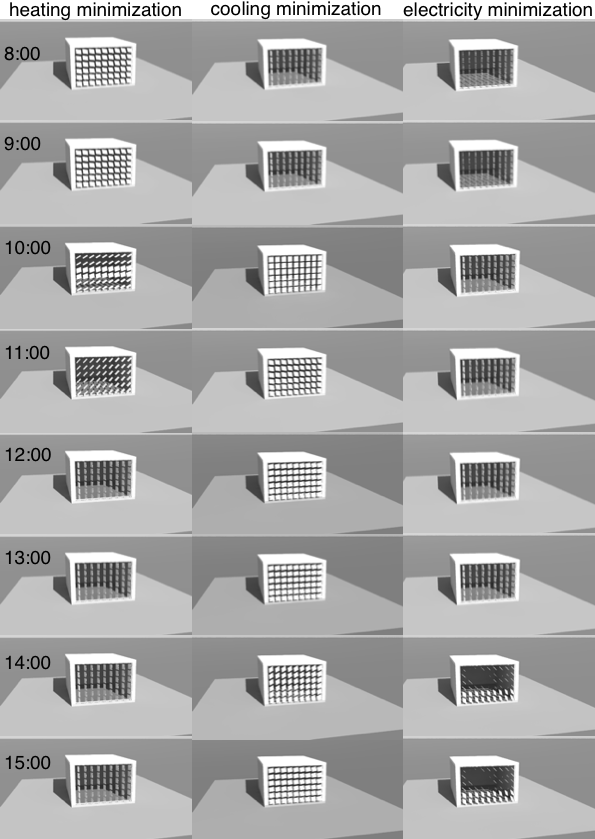
\includegraphics[width=150mm]{graphic/sequence.png}
 \caption{Comparison of the solutions obtained by minimizing the heating, cooling and electricity consumption at the first of February.}
 \label{visualization}
\end{figure}